\section{Auswertung}
\label{sec:Auswertung}

\subsection{Justage der Apperatur}
Um ein möglichst homogenes Magnetfeld einzustellen werden die Shim-Parameter auf 
\begin{align*}
  x =& \num{-1.0}\\
  y =& \num{-5.0}\\
  z =& \num{3.7}\\
  z^2 =& \num{-2.4}
\end{align*}
eingestellt.
Die Lamor-Frequenz wird auf $\omega_{\text{L}} = \SI{21.71585}{\mega\hertz}$ eingestellt.
Die Pulslänge für einen $\SI{90}{\degree}$ Puls wird als $t_{\text{90}}=\SI{2.7}{\micro\second}$ bestimmt.
Für den $\SI{180}{\degree}$ Puls beträgt die Pulslänge $t_{\text{180}}=\SI{5}{\micro\second}$, dass passt mit der 
Annahme überein, dass diese Pulslänge doppelt so lang sein soll. Die Temperatur an der Stelle der Probe beträgt $\SI{22.2}{\celsius}$.

\subsection{Bestimmung der Relaxationszeit $T_{\text{1}}$}
Für die Bestimmung der Relaxationszeit wird die Spannung in abhängigkeit des Pulsabstandes $\tau$ gemessen.
Die gemessenen Daten sind in Tabelle \ref{tab:T1_Data} aufgelistet.
\begin{table}
  \centering
  \caption{Messdaten für die Bestimmung der Relaxationszeit $T_{\text{1}}$.}
  \label{tab:T1_Data}
  \begin{tabular}{c c}
    \toprule
    $\tau$\,/\,$\SI{}{\second}$&U\,/\,$\SI{}{\volt}$\\
    \midrule
    $\num{0.0002}$&$\num{2.09375}$\\
    $\num{0.0005}$&$\num{2.05625}$\\
    $\num{0.0010}$&$\num{1.99375}$\\
    $\num{0.0015}$&$\num{2.03750}$\\
    $\num{0.0025}$&$\num{2.17500}$\\
    $\num{0.0050}$&$\num{2.16250}$\\
    $\num{0.0100}$&$\num{2.15000}$\\
    $\num{0.0150}$&$\num{2.16875}$\\
    $\num{0.0350}$&$\num{2.13125}$\\
    $\num{0.0500}$&$\num{2.10625}$\\
    $\num{0.1000}$&$\num{2.06250}$\\
    $\num{0.3000}$&$\num{1.78125}$\\
    $\num{0.6000}$&$\num{1.38750}$\\
    $\num{0.9000}$&$\num{1.03750}$\\
    $\num{1.5000}$&$\num{0.41750}$\\
    $\num{1.2000}$&$\num{0.69500}$\\
    $\num{1.4000}$&$\num{0.51500}$\\
    $\num{1.6000}$&$\num{0.33750}$\\
    $\num{1.8000}$&$\num{0.15250}$\\
    $\num{2.0000}$&$\num{0.11500}$\\
    $\num{2.2000}$&$\num{0.31500}$\\
    $\num{2.4000}$&$\num{0.32000}$\\
    $\num{2.6000}$&$\num{0.32000}$\\
    $\num{3.0000}$&$\num{0.33000}$\\
    $\num{3.5000}$&$\num{0.33250}$\\
    \bottomrule
  \end{tabular}
\end{table}
An die Daten aus Tabelle \ref{tab:T1_Data} wird die Funktion 
\begin{equation}
  \label{eq:Fit_Funktion_T1T2}
  U(\tau)= U_{\text{0}} \exp{-\frac{\tau}{-T_{\text{1}}}} + U_{\text{1}}
\end{equation}
angepasst.
Die Fitparameter sind
\begin{align*}
  U_{\text{0}} =& \SI{-3.22(21)}{\volt}\\
  U_{\text{1}} =& \SI{1.07(22)}{\volt}\\
  T_{\text{1}} =& \SI{1.92(24)}{\second}.
\end{align*}
Der Fitparameter $T_{\text{1}}$ ist die Relaxationszeit.
Die Messdaten und der Fit sind in Abbildung \ref{fig:T1_Data_fit} zu sehen.
\begin{figure}
  \centering
  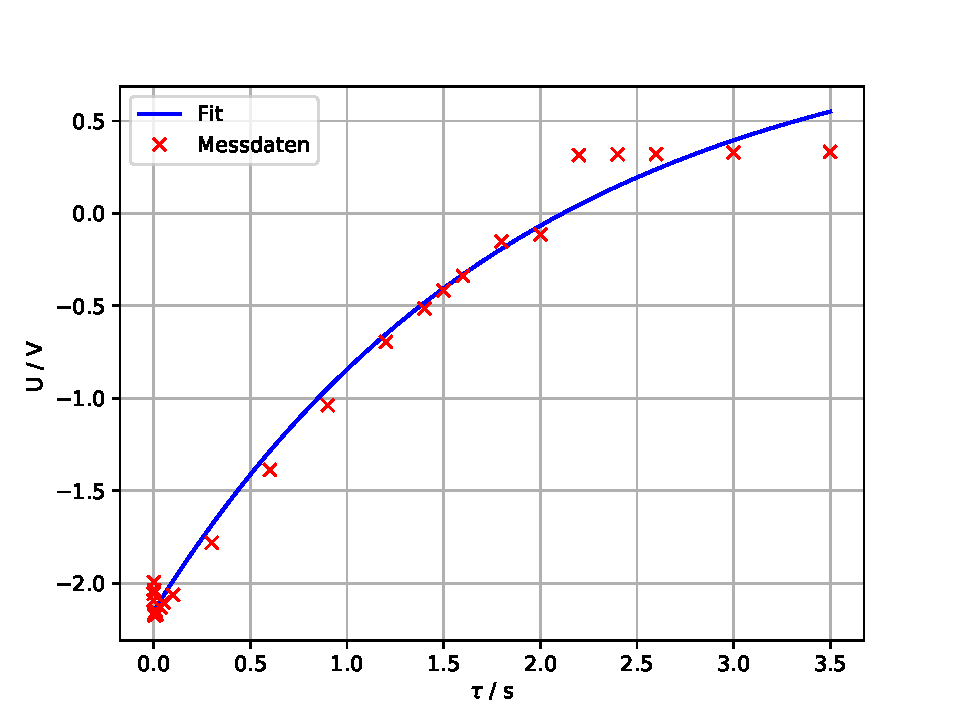
\includegraphics[width = \textwidth, keepaspectratio]{figure/T1_fit.pdf}
  \caption{Messdaten und Fit für die Bestimmung der Relaxationszeit $T_{\text{1}}$.}
  \label{fig:T1_Data_fit}
\end{figure}
\FloatBarrier
\subsection{Bestimmung der Relaxationszeit $T_{\text{2}}$}
In diesem Versuchsteil wird der A-Puls auf $\SI{90}{\degree}$ und der B-Puls auf $\SI{180}{degree}$ eingestellt. Der B-Puls
soll 100 mal wiederholt werden.
Die Periodendauer wird auf den Wert $P=3T_{\text{1}}\approx \SI{6.0}{\second}$ eingestellt. Die damit aufgenommenen Daten sind in 
Abbildung \ref{fig:T2_Data_Fit} dargestellt.
\begin{figure}
  \centering
  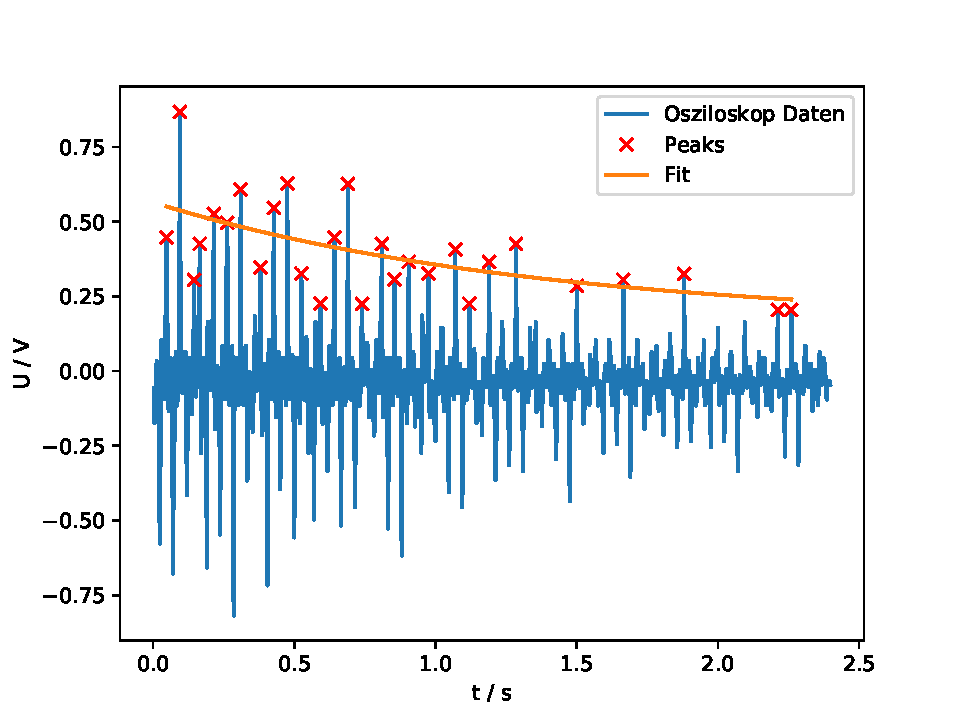
\includegraphics[width = \textwidth, keepaspectratio]{figure/T2_Data_fit.pdf}
  \caption{Peaks und Fit für die Bestimmung der Relaxationszeit $T_{\text{2}}$.}
  \label{fig:T2_Data_Fit}
\end{figure}
Die markierten Peaks aus Abbildung \ref{fig:T2_Data_Fit} wurden mit der Funktion $\texttt{find\_peaks}$ aus der Bibliothek
$\texttt{scipy.signal}$ [Quelle hinzufühgen] ermittelt.
Die Peaks sind in Tabelle \ref{tab:Peaks_T2} aufgelistet.
\begin{table}
  \centering
  \caption{Ermittelte Peaks für die Bestimmung des Fits.}
  \label{tab:Peaks_T2}
  \begin{tabular}{c c}
    \toprule
    $t$\,/\,$\SI{}{\second}$&$U$\,/\,$\SI{}{\volt}$\\
    \midrule
    $\num{0.0475}$&$\num{0.445854}$\\
    $\num{0.095}$&$\num{0.867965}$\\
    $\num{0.145}$&$\num{0.305151}$\\
    $\num{0.165}$&$\num{0.425754}$\\
    $\num{0.215}$&$\num{0.526256}$\\
    $\num{0.2625}$&$\num{0.496106}$\\
    $\num{0.31}$&$\num{0.606658}$\\
    $\num{0.38}$&$\num{0.345352}$\\
    $\num{0.4275}$&$\num{0.546357}$\\
    $\num{0.475}$&$\num{0.626759}$\\
    $\num{0.525}$&$\num{0.325251}$\\
    $\num{0.5925}$&$\num{0.224749}$\\
    $\num{0.6425}$&$\num{0.445854}$\\
    $\num{0.69}$&$\num{0.626759}$\\
    $\num{0.74}$&$\num{0.224749}$\\
    $\num{0.81}$&$\num{0.425754}$\\
    $\num{0.855}$&$\num{0.305151}$\\
    $\num{0.905}$&$\num{0.365452}$\\
    $\num{0.975}$&$\num{0.325251}$\\
    $\num{1.07}$&$\num{0.40691}$\\
    $\num{1.12}$&$\num{0.224749}$\\
    $\num{1.19}$&$\num{0.365452}$\\
    $\num{1.285}$&$\num{0.425754}$\\
    $\num{1.5}$&$\num{0.28505}$\\
    $\num{1.665}$&$\num{0.305151}$\\
    $\num{1.88}$&$\num{0.325251}$\\
    $\num{2.2125}$&$\num{0.204648}$\\
    $\num{2.26}$&$\num{0.204648}$\\
    \bottomrule
  \end{tabular}
\end{table}   
An die Peaks wird die Funktion \eqref{eq:Fit_Funktion_T1T2} angepasst, bei dieser Funktion wird allerdings $T_{\text{1}}$
mit $T_{\text{2}}$ ausgetauscht.
Die Fitparameter sind
\begin{align*}
  U_{\text{0}} =& \SI{0.40(24)}{\volt}\\
  U_{\text{1}} =& \SI{0.16(27)}{\volt}\\
  T_{\text{2}} =& \SI{1.4(18)}{\second}.
\end{align*}
\FloatBarrier
Mit der Carr-Purcell-Methode hätte die Relaxationszeit $T_{\text{2}}$ auch bestimmt werden können, wenn die Pulslänge 
für den $\SI{180}{\degree}$-Puls exakt eingestellt wäre. Da dies aber nicht der Fall ist, kommt er zu einem systematischen
Fehler, dadurch würde die damit bestimmte Relaxationszeit fehlerhaft sein.
Dieser Fehler hebt sich bei der vorherigen Meiboom-Gill-Methode durch die Phasenverschiebung weg.
Das Bild mit dem $T_{\text{2}}$ bestimmt werden 
soll ist die Abbildung \ref{fig:CPM}. 
\begin{figure}
  \centering
  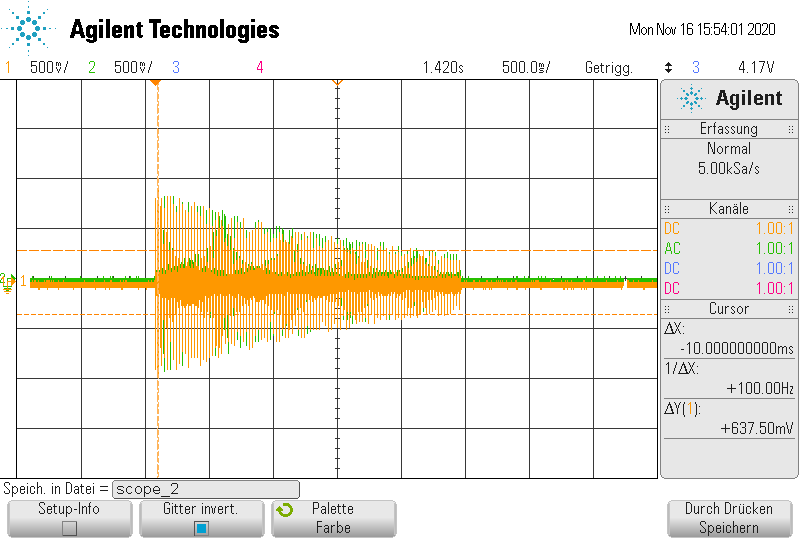
\includegraphics[width = \textwidth,keepaspectratio]{../Bilder/scope_2.png}
  \caption{Bild des Oszilloskopen für die Carr-Purcell-Methode.}
  \label{fig:CPM}
\end{figure}
\FloatBarrier
\subsection{Diffusionsmessung}
Bei diesem Versuchsteil muss der z-Gradient umgepolt und maximiert werden. Die anderen Shim-Parameter bleiben unverändert. 
Um die Diffusionskonstante zu messen wird der A-Puls auf $\SI{90}{\degree}$ und der B-Puls auf $\SI{180}{\degree}$ eingestellt.
Die Anzahl der Pulsewiederholungen von B ist $N=1$. Die Periodendauer wird wieder auf $P=3T_{\text{1}}\approx \SI{6.0}{\second}$ 
eingestellt.
Es wird wieder die Spannungsamplitude in abhängigkeit des Pulsabstandes $\tau$ gemessen.
Die gemessenen Daten sind in Tabelle \ref{tab:Diff_messung} aufgelistet. 
\begin{table}
  \centering
  \caption{Messdaten für die Bestimmung der Diffusionskonstante.}
  \label{tab:Diff_messung}
  \begin{tabular}{c c}
    \toprule
    $\tau$\,/\,$\SI{}{\second}$&$U$\,/\,$\SI{}{\volt}$\\
    $\num{0.0002}$&$\num{1.16250}$\\
    $\num{0.0010}$&$\num{1.19375}$\\
    $\num{0.0050}$&$\num{1.11875}$\\
    $\num{0.0100}$&$\num{0.70625}$\\
    $\num{0.0133}$&$\num{0.34375}$\\
    $\num{0.0140}$&$\num{0.28750}$\\
    $\num{0.0150}$&$\num{0.20000}$\\
    $\num{0.0160}$&$\num{0.16875}$\\
    $\num{0.0170}$&$\num{0.12500}$\\
    $\num{0.0180}$&$\num{0.08750}$\\
    $\num{0.0115}$&$\num{0.52500}$\\
    $\num{0.0060}$&$\num{1.00625}$\\
    $\num{0.0075}$&$\num{0.96250}$\\
    $\num{0.0085}$&$\num{0.88750}$\\
    $\num{0.0138}$&$\num{0.33125}$\\
    $\num{0.0122}$&$\num{0.41250}$\\
    \bottomrule
  \end{tabular}
\end{table}
